\documentclass{standalone}
\usepackage{tikz}
\usetikzlibrary{patterns, positioning}


\begin{document}
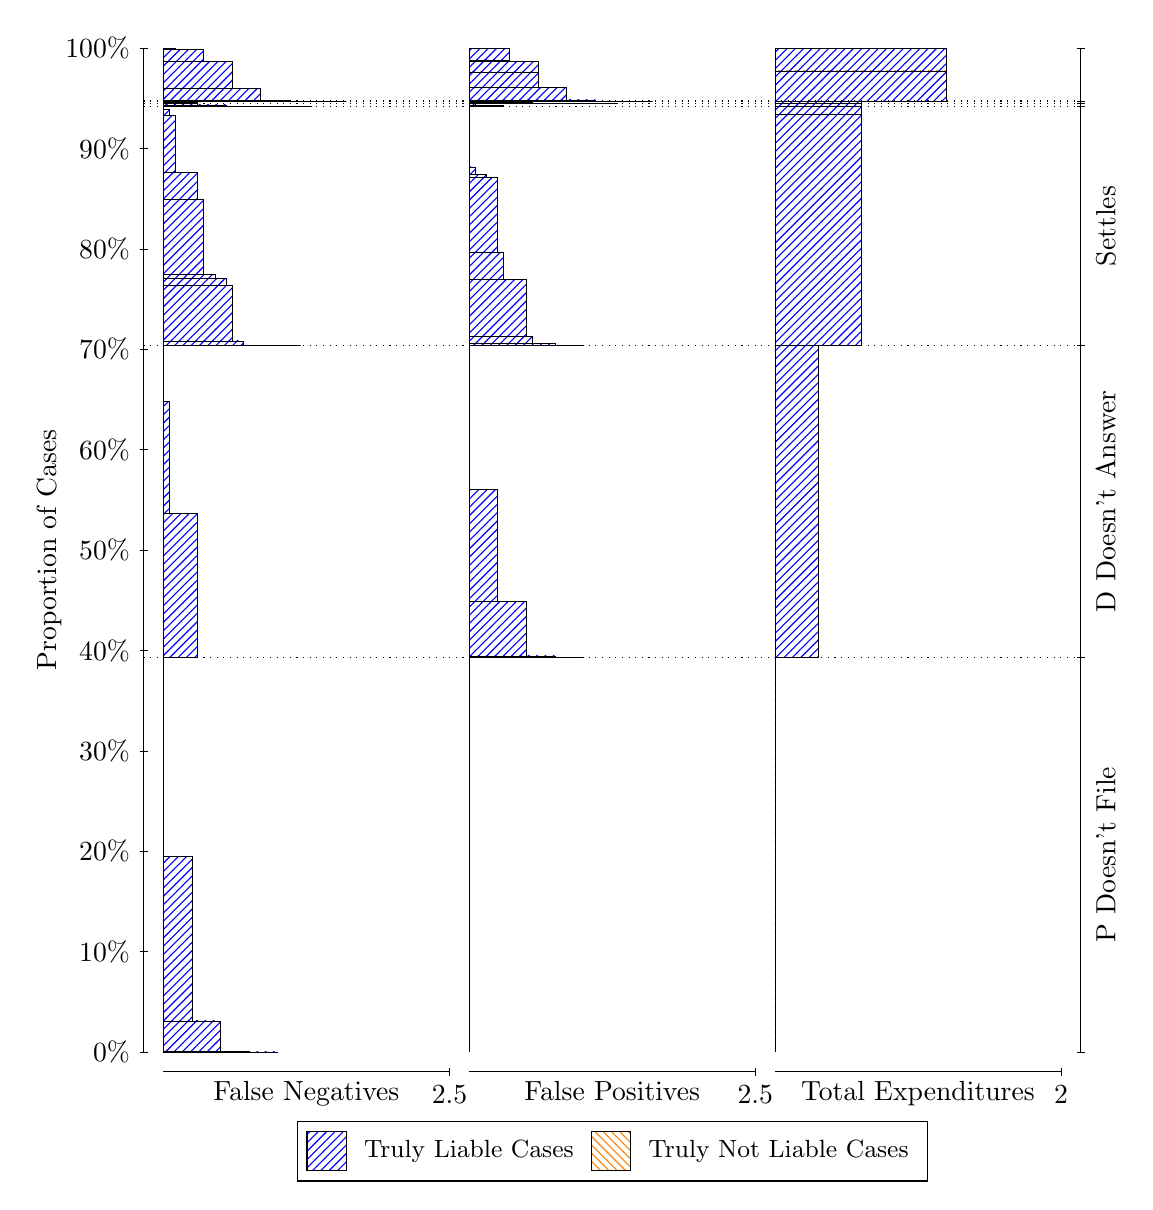
\begin{tikzpicture}
\draw[black, very thin] (1.5,1.75) -- (1.5,14.5);
\node[rotate=90, text=black, anchor=center] at (0.3, 8.125) {Proportion of Cases};
\draw[black, very thin] (1.45,1.75) -- (1.55,1.75);
\node[text=black, anchor=east] at (1.45, 1.75) {0\%};
\draw[black, very thin] (1.45,3.025) -- (1.55,3.025);
\node[text=black, anchor=east] at (1.45, 3.025) {10\%};
\draw[black, very thin] (1.45,4.3) -- (1.55,4.3);
\node[text=black, anchor=east] at (1.45, 4.3) {20\%};
\draw[black, very thin] (1.45,5.575) -- (1.55,5.575);
\node[text=black, anchor=east] at (1.45, 5.575) {30\%};
\draw[black, very thin] (1.45,6.85) -- (1.55,6.85);
\node[text=black, anchor=east] at (1.45, 6.85) {40\%};
\draw[black, very thin] (1.45,8.125) -- (1.55,8.125);
\node[text=black, anchor=east] at (1.45, 8.125) {50\%};
\draw[black, very thin] (1.45,9.4) -- (1.55,9.4);
\node[text=black, anchor=east] at (1.45, 9.4) {60\%};
\draw[black, very thin] (1.45,10.675) -- (1.55,10.675);
\node[text=black, anchor=east] at (1.45, 10.675) {70\%};
\draw[black, very thin] (1.45,11.95) -- (1.55,11.95);
\node[text=black, anchor=east] at (1.45, 11.95) {80\%};
\draw[black, very thin] (1.45,13.225) -- (1.55,13.225);
\node[text=black, anchor=east] at (1.45, 13.225) {90\%};
\draw[black, very thin] (1.45,14.5) -- (1.55,14.5);
\node[text=black, anchor=east] at (1.45, 14.5) {100\%};

\draw[black, very thin] (13.4,1.75) -- (13.4,14.5);
\draw[black, very thin] (13.35,1.75) -- (13.45,1.75);
\node[anchor=west] at (13.35, 1.75) {};
\draw[black, very thin] (13.35,6.7597) -- (13.45,6.7597);
\node[anchor=west] at (13.35, 6.7597) {};
\draw[black, very thin] (13.35,10.723) -- (13.45,10.723);
\node[anchor=west] at (13.35, 10.723) {};
\draw[black, very thin] (13.35,13.755) -- (13.45,13.755);
\node[anchor=west] at (13.35, 13.755) {};
\draw[black, very thin] (13.35,13.793) -- (13.45,13.793);
\node[anchor=west] at (13.35, 13.793) {};
\draw[black, very thin] (13.35,13.827) -- (13.45,13.827);
\node[anchor=west] at (13.35, 13.827) {};
\draw[black, very thin] (13.35,14.5) -- (13.45,14.5);
\node[anchor=west] at (13.35, 14.5) {};

\draw[black, very thin, pattern color=blue, pattern=north east lines] (1.75,1.75) rectangle (3.2033,1.75);
\draw[black, very thin, pattern color=blue, pattern=north east lines] (1.75,1.75) rectangle (2.84,1.7533);
\draw[black, very thin, pattern color=blue, pattern=north east lines] (1.75,1.7533) rectangle (2.4767,2.1443);
\draw[black, very thin, pattern color=blue, pattern=north east lines] (1.75,2.1443) rectangle (2.1133,4.23);
\draw[black, very thin, pattern color=orange, pattern=north west lines] (1.75,4.23) rectangle (1.75,4.23);
\draw[black, very thin, pattern color=blue, pattern=north east lines] (1.75,4.23) rectangle (1.75,6.7597);
\draw[black, very thin, pattern color=blue, pattern=north east lines] (1.75,6.7597) rectangle (2.186,8.5867);
\draw[black, very thin, pattern color=blue, pattern=north east lines] (1.75,8.5867) rectangle (1.8227,10.01);
\draw[black, very thin, pattern color=orange, pattern=north west lines] (1.75,10.01) rectangle (1.75,10.01);
\draw[black, very thin, pattern color=blue, pattern=north east lines] (1.75,10.01) rectangle (1.75,10.723);
\draw[black, very thin, pattern color=blue, pattern=north east lines] (1.75,10.723) rectangle (3.494,10.723);
\draw[black, very thin, pattern color=blue, pattern=north east lines] (1.75,10.723) rectangle (3.1307,10.725);
\draw[black, very thin, pattern color=blue, pattern=north east lines] (1.75,10.725) rectangle (2.9127,10.727);
\draw[black, very thin, pattern color=blue, pattern=north east lines] (1.75,10.727) rectangle (2.7673,10.782);
\draw[black, very thin, pattern color=blue, pattern=north east lines] (1.75,10.782) rectangle (2.622,11.488);
\draw[black, very thin, pattern color=blue, pattern=north east lines] (1.75,11.488) rectangle (2.5493,11.579);
\draw[black, very thin, pattern color=blue, pattern=north east lines] (1.75,11.579) rectangle (2.404,11.621);
\draw[black, very thin, pattern color=blue, pattern=north east lines] (1.75,11.621) rectangle (2.2587,12.577);
\draw[black, very thin, pattern color=blue, pattern=north east lines] (1.75,12.577) rectangle (2.186,12.919);
\draw[black, very thin, pattern color=blue, pattern=north east lines] (1.75,12.919) rectangle (2.0407,12.92);
\draw[black, very thin, pattern color=blue, pattern=north east lines] (1.75,12.92) rectangle (1.8953,13.641);
\draw[black, very thin, pattern color=blue, pattern=north east lines] (1.75,13.641) rectangle (1.8227,13.727);
\draw[black, very thin, pattern color=orange, pattern=north west lines] (1.75,13.727) rectangle (1.75,13.727);
\draw[black, very thin, pattern color=blue, pattern=north east lines] (1.75,13.727) rectangle (1.75,13.755);
\draw[black, very thin, pattern color=blue, pattern=north east lines] (1.75,13.755) rectangle (3.6393,13.755);
\draw[black, very thin, pattern color=blue, pattern=north east lines] (1.75,13.755) rectangle (3.276,13.755);
\draw[black, very thin, pattern color=blue, pattern=north east lines] (1.75,13.755) rectangle (2.9127,13.756);
\draw[black, very thin, pattern color=blue, pattern=north east lines] (1.75,13.756) rectangle (2.5493,13.779);
\draw[black, very thin, pattern color=blue, pattern=north east lines] (1.75,13.779) rectangle (2.186,13.793);
\draw[black, very thin, pattern color=orange, pattern=north west lines] (1.75,13.793) rectangle (1.75,13.793);
\draw[black, very thin, pattern color=blue, pattern=north east lines] (1.75,13.793) rectangle (2.186,13.807);
\draw[black, very thin, pattern color=blue, pattern=north east lines] (1.75,13.807) rectangle (1.8227,13.827);
\draw[black, very thin, pattern color=orange, pattern=north west lines] (1.75,13.827) rectangle (1.75,13.827);
\draw[black, very thin, pattern color=blue, pattern=north east lines] (1.75,13.827) rectangle (1.75,13.827);
\draw[black, very thin, pattern color=blue, pattern=north east lines] (1.75,13.827) rectangle (4.0753,13.827);
\draw[black, very thin, pattern color=blue, pattern=north east lines] (1.75,13.827) rectangle (3.712,13.827);
\draw[black, very thin, pattern color=blue, pattern=north east lines] (1.75,13.827) rectangle (3.3487,13.836);
\draw[black, very thin, pattern color=blue, pattern=north east lines] (1.75,13.836) rectangle (2.9853,13.992);
\draw[black, very thin, pattern color=blue, pattern=north east lines] (1.75,13.992) rectangle (2.622,14.33);
\draw[black, very thin, pattern color=blue, pattern=north east lines] (1.75,14.33) rectangle (2.2587,14.486);
\draw[black, very thin, pattern color=blue, pattern=north east lines] (1.75,14.486) rectangle (1.8953,14.5);
\draw[black, very thin, pattern color=orange, pattern=north west lines] (1.75,14.5) rectangle (1.75,14.5);
\draw[black, very thin, pattern color=blue, pattern=north east lines] (1.75,14.5) rectangle (1.75,14.5);
\draw[black, very thin, pattern color=orange, pattern=north west lines] (5.6333,1.75) rectangle (5.6333,1.75);
\draw[black, very thin, pattern color=blue, pattern=north east lines] (5.6333,1.75) rectangle (5.6333,6.7597);
\draw[black, very thin, pattern color=orange, pattern=north west lines] (5.6333,6.7597) rectangle (7.0867,6.7597);
\draw[black, very thin, pattern color=blue, pattern=north east lines] (5.6333,6.7597) rectangle (7.0867,6.7597);
\draw[black, very thin, pattern color=blue, pattern=north east lines] (5.6333,6.7597) rectangle (6.7233,6.7817);
\draw[black, very thin, pattern color=blue, pattern=north east lines] (5.6333,6.7817) rectangle (6.36,7.4729);
\draw[black, very thin, pattern color=blue, pattern=north east lines] (5.6333,7.4729) rectangle (5.9967,8.8964);
\draw[black, very thin, pattern color=blue, pattern=north east lines] (5.6333,8.8964) rectangle (5.6333,10.723);
\draw[black, very thin, pattern color=orange, pattern=north west lines] (5.6333,10.723) rectangle (7.0867,10.723);
\draw[black, very thin, pattern color=blue, pattern=north east lines] (5.6333,10.723) rectangle (7.0867,10.723);
\draw[black, very thin, pattern color=orange, pattern=north west lines] (5.6333,10.723) rectangle (6.796,10.723);
\draw[black, very thin, pattern color=blue, pattern=north east lines] (5.6333,10.723) rectangle (6.796,10.726);
\draw[black, very thin, pattern color=blue, pattern=north east lines] (5.6333,10.726) rectangle (6.7233,10.751);
\draw[black, very thin, pattern color=blue, pattern=north east lines] (5.6333,10.751) rectangle (6.4327,10.837);
\draw[black, very thin, pattern color=blue, pattern=north east lines] (5.6333,10.837) rectangle (6.36,11.559);
\draw[black, very thin, pattern color=orange, pattern=north west lines] (5.6333,11.559) rectangle (6.2147,11.559);
\draw[black, very thin, pattern color=blue, pattern=north east lines] (5.6333,11.559) rectangle (6.2147,11.56);
\draw[black, very thin, pattern color=blue, pattern=north east lines] (5.6333,11.56) rectangle (6.0693,11.902);
\draw[black, very thin, pattern color=blue, pattern=north east lines] (5.6333,11.902) rectangle (5.9967,12.858);
\draw[black, very thin, pattern color=blue, pattern=north east lines] (5.6333,12.858) rectangle (5.8513,12.9);
\draw[black, very thin, pattern color=blue, pattern=north east lines] (5.6333,12.9) rectangle (5.706,12.991);
\draw[black, very thin, pattern color=blue, pattern=north east lines] (5.6333,12.991) rectangle (5.6333,13.755);
\draw[black, very thin, pattern color=orange, pattern=north west lines] (5.6333,13.755) rectangle (6.0693,13.755);
\draw[black, very thin, pattern color=blue, pattern=north east lines] (5.6333,13.755) rectangle (6.0693,13.769);
\draw[black, very thin, pattern color=blue, pattern=north east lines] (5.6333,13.769) rectangle (5.706,13.792);
\draw[black, very thin, pattern color=blue, pattern=north east lines] (5.6333,13.792) rectangle (5.6333,13.793);
\draw[black, very thin, pattern color=orange, pattern=north west lines] (5.6333,13.793) rectangle (7.5227,13.793);
\draw[black, very thin, pattern color=blue, pattern=north east lines] (5.6333,13.793) rectangle (7.5227,13.793);
\draw[black, very thin, pattern color=blue, pattern=north east lines] (5.6333,13.793) rectangle (7.1593,13.793);
\draw[black, very thin, pattern color=blue, pattern=north east lines] (5.6333,13.793) rectangle (6.796,13.793);
\draw[black, very thin, pattern color=blue, pattern=north east lines] (5.6333,13.793) rectangle (6.4327,13.814);
\draw[black, very thin, pattern color=blue, pattern=north east lines] (5.6333,13.814) rectangle (6.0693,13.827);
\draw[black, very thin, pattern color=orange, pattern=north west lines] (5.6333,13.827) rectangle (7.9587,13.827);
\draw[black, very thin, pattern color=blue, pattern=north east lines] (5.6333,13.827) rectangle (7.9587,13.827);
\draw[black, very thin, pattern color=orange, pattern=north west lines] (5.6333,13.827) rectangle (7.5953,13.827);
\draw[black, very thin, pattern color=blue, pattern=north east lines] (5.6333,13.827) rectangle (7.5953,13.827);
\draw[black, very thin, pattern color=orange, pattern=north west lines] (5.6333,13.827) rectangle (7.232,13.827);
\draw[black, very thin, pattern color=blue, pattern=north east lines] (5.6333,13.827) rectangle (7.232,13.841);
\draw[black, very thin, pattern color=blue, pattern=north east lines] (5.6333,13.841) rectangle (6.8687,13.997);
\draw[black, very thin, pattern color=orange, pattern=north west lines] (5.6333,13.997) rectangle (6.8687,13.997);
\draw[black, very thin, pattern color=blue, pattern=north east lines] (5.6333,13.997) rectangle (6.8687,13.998);
\draw[black, very thin, pattern color=blue, pattern=north east lines] (5.6333,13.998) rectangle (6.5053,14.198);
\draw[black, very thin, pattern color=orange, pattern=north west lines] (5.6333,14.198) rectangle (6.5053,14.198);
\draw[black, very thin, pattern color=blue, pattern=north east lines] (5.6333,14.198) rectangle (6.5053,14.335);
\draw[black, very thin, pattern color=blue, pattern=north east lines] (5.6333,14.335) rectangle (6.142,14.348);
\draw[black, very thin, pattern color=blue, pattern=north east lines] (5.6333,14.348) rectangle (6.142,14.491);
\draw[black, very thin, pattern color=blue, pattern=north east lines] (5.6333,14.491) rectangle (5.7787,14.491);
\draw[black, very thin, pattern color=blue, pattern=north east lines] (5.6333,14.491) rectangle (5.7787,14.5);
\draw[black, very thin, pattern color=blue, pattern=north east lines] (5.6333,14.5) rectangle (5.6333,14.5);
\draw[black, very thin, pattern color=orange, pattern=north west lines] (9.5167,1.75) rectangle (9.5167,1.75);
\draw[black, very thin, pattern color=blue, pattern=north east lines] (9.5167,1.75) rectangle (9.5167,6.7597);
\draw[black, very thin, pattern color=orange, pattern=north west lines] (9.5167,6.7597) rectangle (10.062,6.7597);
\draw[black, very thin, pattern color=blue, pattern=north east lines] (9.5167,6.7597) rectangle (10.062,10.723);
\draw[black, very thin, pattern color=orange, pattern=north west lines] (9.5167,10.723) rectangle (10.607,10.723);
\draw[black, very thin, pattern color=blue, pattern=north east lines] (9.5167,10.723) rectangle (10.607,13.657);
\draw[black, very thin, pattern color=orange, pattern=north west lines] (9.5167,13.657) rectangle (10.607,13.657);
\draw[black, very thin, pattern color=blue, pattern=north east lines] (9.5167,13.657) rectangle (10.607,13.755);
\draw[black, very thin, pattern color=orange, pattern=north west lines] (9.5167,13.755) rectangle (10.607,13.755);
\draw[black, very thin, pattern color=blue, pattern=north east lines] (9.5167,13.755) rectangle (10.607,13.793);
\draw[black, very thin, pattern color=orange, pattern=north west lines] (9.5167,13.793) rectangle (10.607,13.793);
\draw[black, very thin, pattern color=blue, pattern=north east lines] (9.5167,13.793) rectangle (10.607,13.827);
\draw[black, very thin, pattern color=orange, pattern=north west lines] (9.5167,13.827) rectangle (11.697,13.827);
\draw[black, very thin, pattern color=blue, pattern=north east lines] (9.5167,13.827) rectangle (11.697,14.21);
\draw[black, very thin, pattern color=orange, pattern=north west lines] (9.5167,14.21) rectangle (11.697,14.21);
\draw[black, very thin, pattern color=blue, pattern=north east lines] (9.5167,14.21) rectangle (11.697,14.5);
\draw[black, dotted] (1.5,6.7597) -- (13.4,6.7597);
\draw[black, dotted] (1.5,10.723) -- (13.4,10.723);
\draw[black, dotted] (1.5,13.755) -- (13.4,13.755);
\draw[black, dotted] (1.5,13.793) -- (13.4,13.793);
\draw[black, dotted] (1.5,13.827) -- (13.4,13.827);
\draw[black, very thin] (1.75,1.5) -- (5.3833,1.5);
\node[text=black, anchor=north] at (3.5667, 1.5) {False Negatives};
\draw[black, very thin] (5.3833,1.45) -- (5.3833,1.55);
\node[text=black, anchor=north] at (5.3833, 1.45) {2.5};

\draw[black, very thin] (5.6333,1.5) -- (9.2667,1.5);
\node[text=black, anchor=north] at (7.45, 1.5) {False Positives};
\draw[black, very thin] (9.2667,1.45) -- (9.2667,1.55);
\node[text=black, anchor=north] at (9.2667, 1.45) {2.5};

\draw[black, very thin] (9.5167,1.5) -- (13.15,1.5);
\node[text=black, anchor=north] at (11.333, 1.5) {Total Expenditures};
\draw[black, very thin] (13.15,1.45) -- (13.15,1.55);
\node[text=black, anchor=north] at (13.15, 1.45) {2};

\node[text=black, centered, rotate=90] at (13.72, 4.2548) {P Doesn't File};
\node[text=black, centered, rotate=90] at (13.72, 8.7416) {D Doesn't Answer};
\node[text=black, centered, rotate=90] at (13.72, 12.239) {Settles};




\draw (7.449999999999999,1.5) node[draw=none] (baseCoordinate) {};
\begin{scope}[align=center]
        \matrix[scale=0.5, draw=black, below=0.5cm of baseCoordinate, nodes={draw}, column sep=0.1cm]{
            \node[rectangle, draw, minimum width=0.5cm, minimum height=0.5cm, pattern color=blue, pattern=north east lines] {}; &
            \node[draw=none, font=\small, text=black] (B) {Truly Liable Cases}; &
            \node[rectangle, draw, minimum width=0.5cm, minimum height=0.5cm, pattern color=orange, pattern=north west lines] {}; &
            \node[draw=none, font=\small, text=black] (B) {Truly Not Liable Cases}; \\
            };
\end{scope}

\end{tikzpicture}
\end{document}